\section{Durchführung}
\label{sec:Durchführung}

\subsection{Versuchsaufbau}
\label{sec:Versuchsaufbau}

\begin{figure}
	\caption{prinzipieller Versuchsaufbau}
	\label{fig:aufbauamk}
	\centering
	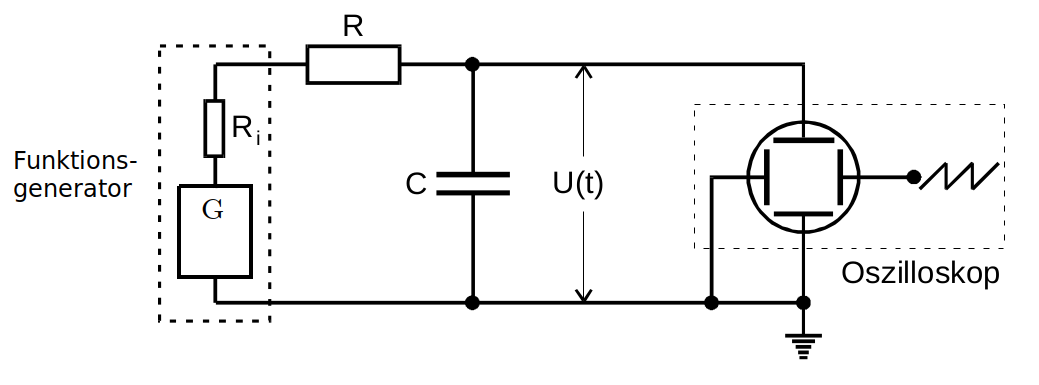
\includegraphics[width=0.7\textwidth]{bilder/generator.png}
\end{figure}

Der prinzipielle Versuchsaufbau ist in Abbildung \ref{fig:aufbauamk} dargestellt.
Dieser entspricht einem Funktionsgenerator, einem RC-Glied sowie einem Zweikanal-Oszilloskop.
An dem Generator lassen sich die Spannungsfrequenzen sowie verschiedene Spannungs
typen - wie beispielsweise die verwendete Rechteck-, Sinus- oder Dreiecksspannung - einstellen.
Außerdem wird dem Funktionsgenerator ein Innenwiderstand $R_{\text{i}}$ zugeordnet, der allerdings unbekannt ist, ebenso wie der ohmsche Widerstand $R$ und die Kapazität $C$ des RC-Gliedes.
Auf dem Zweikanal-Oszilloskop kann die Kondensatorspannung sowie die Generatorspannung aufgezeichnet werden.

\subsection{Versuchsdurchführung}
\label{sec:Versuchsdurchführung}

Wie schon in der Zielsetzung \ref{sec:Zielsetzung} angesprochen soll in diesem Versuch die
Zeitkonstante $RC$ bestimmt werden.
Dazu werden drei verschiedene Methoden verwendet.
Des Weiteren wird gezeigt, dass ein RC-Glied einem Integrationsglied entspricht.

Bei der ersten Methode bestimmt man die Zeitkonstante $RC$ durch Beobachtung der Relaxationsvorgämnge mit dem Oszilloskop.
Zuerst wird am Generator eine Rechteckspannung eingestellt.
Die Kondensatorspannung wird auf den ersten Kanal des Oszilloskops gegeben, auf welchem - durch
die Rechteckspannung bedingte - Auflade- und Entladekurven zu sehen sind.
Daraufhin wird die Frequenz der Rechteckspannung und der Triggerpegel solange variiert, bis
auf dem Oszilloskop eine Entladekurve zu sehen ist, auf der die Kondensatorspannung während der
Aufzeichnungszeit um einen Faktor 5 bis 10 sinkt \cite{Anleitung}.
Nachdem die Entladekurve auf dem Oszilloskop dargestellt ist, können mit der Cursor-Funkton
des Oszilloskops 5-10 Messwerte der Kondensatorspannung $U_{\text{C}}$ sowie der Zeit $t$
abgelesen werden.
Des Weiteren muss noch der Spannungsnullpunkt $U_0$ ermittelt werden.
Hierzu wählt man auf dem Generator eine Spannungsfrequenz $\omega_0$ für die gilt
$\omega_0 \ll \frac{1}{RC}$, damit gilt $U_{\text{C}} \approx U_0$.


Die Messwerte für die zweite und dritte Methode zur Bestimmung der Zeitkonstanten $RC$ werden
in einem Messdurchgang bestimmt.
Bei diesem ist der Aufbau unverändert, außer, dass man zusätzlich die Generatorspannung auf den zweiten Eingang des Oszilloskops gibt und eine Sinusspannung eingestellt wird.
Für die zweite Methode bestimmt man 15 Messwerte für die Spannungsamplitude der Kondensatorspannung mit der zugehörigen Frequenz. Zu ergänzen ist hier, dass die Frequenzen logarithmisch im Bereich von $4 \si{\Hz}$ bis $10000 \si{\Hz}$ variiert werden.
Parallel dazu %gibt es Hummer und Kaviar...
werden für die dritte Methode die zeitlichen Abstände der Nulldurchgänge von Kondensatorspannung und Generatorspannung bestimmt.
Die Bestimmung der Messwerte wird erneut mit der Cursor-Funktion des Oszilloskops realisiert.
Außerdem wird jeweils die Amplitude der Kondensatorspannung notiert.
%... den Champagner hab ich ganz vergessen

Zuletzt soll gezeigt werden, dass ein RC-Glied als Integrationsglied dient.
Hierzu wird bei unverändertem Aufbau eine Frequenz $\omega_1$ eingestellt, für die $\omega_1 \gg RC$ gilt. Dann kann am Generator der Reihe nach eine Rechteck-, Sinus- sowie Dreiecksspannung eingestellt und die auf dem Oszilloskop dargestellten Spannungsverläufe von Generatorspannung und Kondensatorspannung gespeichert werden.
